\documentclass[letterpaper, 10 pt, conference]{ieeeconf}

%\let\labelindent\relax
%\IEEEoverridecommandlockouts
%\overrideIEEEmargins

%floats and figures
\usepackage{graphics}
\usepackage[pdftex]{graphicx}
\usepackage[font={small}]{caption}
\usepackage{subcaption}
%\usepackage[center]{subfigure} %DONT USE BOTH SUBCAPTION AND SUBFIGURE
%\DeclareGraphicsExtensions{.pdf,.png,.jpg}
%\usepackage{overpic}
%\usepackage[rightcaption]{sidecap}
%\usepackage{pbox}

%Math Stuff
\usepackage{mathtools}
\usepackage{amsmath, amssymb, amscd}
%\usepackage{ wasysym } %special symbols
\usepackage{amsfonts}
\usepackage{mathptmx}       % selects Times Roman as basic font
\DeclareMathAlphabet{\mathcal}{OMS}{lmsy}{m}{n}
\DeclareSymbolFont{largesymbols}{OMX}{cmex}{m}{n}
\usepackage{algorithm}
\usepackage{algorithmicx}
%\usepackage{algorithm}
%\usepackage{algpseudocode}
% \usepackage[ruled,vlined,linesnumbered]{algorithm2e}
\usepackage{ textcomp } %for getting text tilde

%Table Stuff
\usepackage{array} %for table entries to be in center of cell
\usepackage{tabularx}
\usepackage{multicol}
\usepackage{multirow}

%DOCUMENT WIDE
\usepackage{times} % assumes new font selection scheme installed
\usepackage{xspace}
\usepackage[english]{babel} %for hyphenation rules
%\usepackage{flushend}%balance columns on last page
\usepackage{fixltx2e} %fix latex issue across versions
\usepackage{bm}
\usepackage{units}

\usepackage{makeidx}
% \usepackage{enumitem}
\usepackage[yyyymmdd,hhmmss]{datetime}
\usepackage[english]{babel}

%Bibliography and cross-ref
\makeatletter
\let\NAT@parse\undefined
\makeatother
\usepackage[numbers]{natbib}
\renewcommand{\bibfont}{\footnotesize}
% \usepackage{cite} %DONT USE NATBIB AND CITE TOGETHER

%hyperlinking
\usepackage{url}
\makeatletter
\g@addto@macro{\UrlBreaks}{\UrlOrds}
\makeatother
\usepackage{color}
\usepackage[usenames,dvipsnames, table]{xcolor}
\usepackage[pdfborder={0 0 0.5}]{hyperref}
\hypersetup{
    colorlinks=true,
    linkcolor=blue,
    citecolor=black,
    filecolor=cyan,
    urlcolor=blue
}


%=======U S E R  D E F I N E D  M A C R O S=======
% \newcommand{\bibhref}[2]{#2}
\newcommand{\todo}[1]{\textcolor{red}{[ToDo:#1]}}
\newcommand{\tocite}[1]{\textcolor{red}{[cite]}}
\newcommand{\ignore}[1]{}

% Usage:
% \figlabel{myfigure} creates \label{fig:myfigure}
% \figref{myfigure} references it
\newcommand{\figlabel}[1]{\label{fig:#1}}
\newcommand{\figref}[1]{Figure~\ref{fig:#1}}

% Usage:
% \seclabel{mysection} creates \label{sec:mysection}
% \secref{mysection} references it
\newcommand{\seclabel}[1]{\label{sec:#1}}
\newcommand{\secref}[1]{Section~\ref{sec:#1}}

% Usage:
% \tablabel{mytable} creates \label{tab:mytable}
% \tabref{mytable} references it
\newcommand{\tablabel}[1]{\label{tab:#1}}
\newcommand{\tabref}[1]{Table~\ref{tab:#1}}

% use this command instead of writing "da Vinci" so it's never split 
\newcommand{\davinci}{da~Vinci\xspace}

\usepackage{blindtext}

%===============================================================
\title{\LARGE \bf
Pixels to Primitives: Learning Sub-Task Level Semantic Segmentation \\
of Multi-Step Task Trajectories from Video with Deep Learning }
% Pixels to Primitives (P2P)

\author{%
Adithyavairavan Murali*, Animesh Garg*, Sanjay Krishnan*, Florian Pokorny,\\ 
Pieter Abbeel, Trevor Darrell, Ken Goldberg \quad {\textcolor{blue}{[v0.1, \today\,\currenttime]}}
\thanks{\hrule \vspace{5pt} * The authors contributed equally to the paper}%
\thanks{EECS \& IEOR, University of California, Berkeley CA USA; \texttt{\{adithya\_murali, animesh.garg, sanjaykrishnan, ftpokorny, pabbeel, trevor, goldberg\}@berkeley.edu}}%
% \thanks{$^{1}$EECS, University of California, Berkeley; {\{sanjaykrishnan, adithya\_murali\}@berkeley.edu}}%
% \thanks{$^{2}$IEOR and EECS, University of California, Berkeley; {\{animesh.garg, goldberg\}@berkeley.edu}}%
}
\IEEEoverridecommandlockouts %to enable thanks to appear
\newcommand{\sys}{\textsf{TSC+VIS}\xspace}

\begin{document}

\maketitle

\begin{abstract}
Segmentation is an important first step in analyzing long running robotic tasks. For reliable results, it is important to consider both visual and kinematic data, as visual data provides important information about the state of the workspace. 
Existing unsupervised segmentation methodologies are limited in the ways they can leverage visual data and rely on annotations or complete knowledge of all objects in the world. In this paper, we propose a framework that takes a step towards unsupervised segmentation of robotic demonstrations using raw video (i.e., pixel data). 
We identify key transition events in kinematic data, cluster transitions together using visual data, and then identify segments of the raw video corresponding to these clusters of transition events. 
The resulting video segments can be used to design error recovery actions, parameter tuning, action classification, 
and operator skill assessment. 
\todo{Our results on x suggest y}
\end{abstract} 

\section{Introduction}
Segmenting demonstrations of a multistep task is an important first step in a number of robot learning applications: skill-learning \cite{calinon2010learning, kruger2010learning, konidaris2011robot}, learning from demonstrations \cite{Niekum2015learning}, reward function parametrization \cite{hanlearning}, and automation of surgical subtasks \cite{murali2015learning}.
One approach is manual annotation, which can be time-consuming and error-prone if inconsistent.
Therefore, it is desirable to algorithmically extract segments from unlabled data.
Such algorithms fall into two broad categories: (1) dictionary-based, (2) and unsupervised.
Dictionary-based algorithms set a pre-defined vocabulary of primitives \emph{a priori} and decompose new trajectories in terms of the primitives; and this approach has been widely applied in the analysis of robotic surgery \cite{lea15improved,zappella2013surgical}.

However, the key challenge in using a dictionary-based approach is building the dictionary of primitives. 
Overly specific primitives may not cover all of the actions seen in a set of demonstrations, while overly general primitives may miss task-specific structure.
Unsupervised techniques can avoid dependence on a pre-defined set of primitives.
Unsupervised methods typically assume some generative mixture model for the data, e.g., locally Gaussian segments, and fit trajectories to this model grouping together locally similar points \cite{calinon2010learning, krishnan2015tsc, calinon2004stochastic, kruger2010learning, fox2009nonparametric, oh2005learning}.


\begin{figure}[ht]
\centering
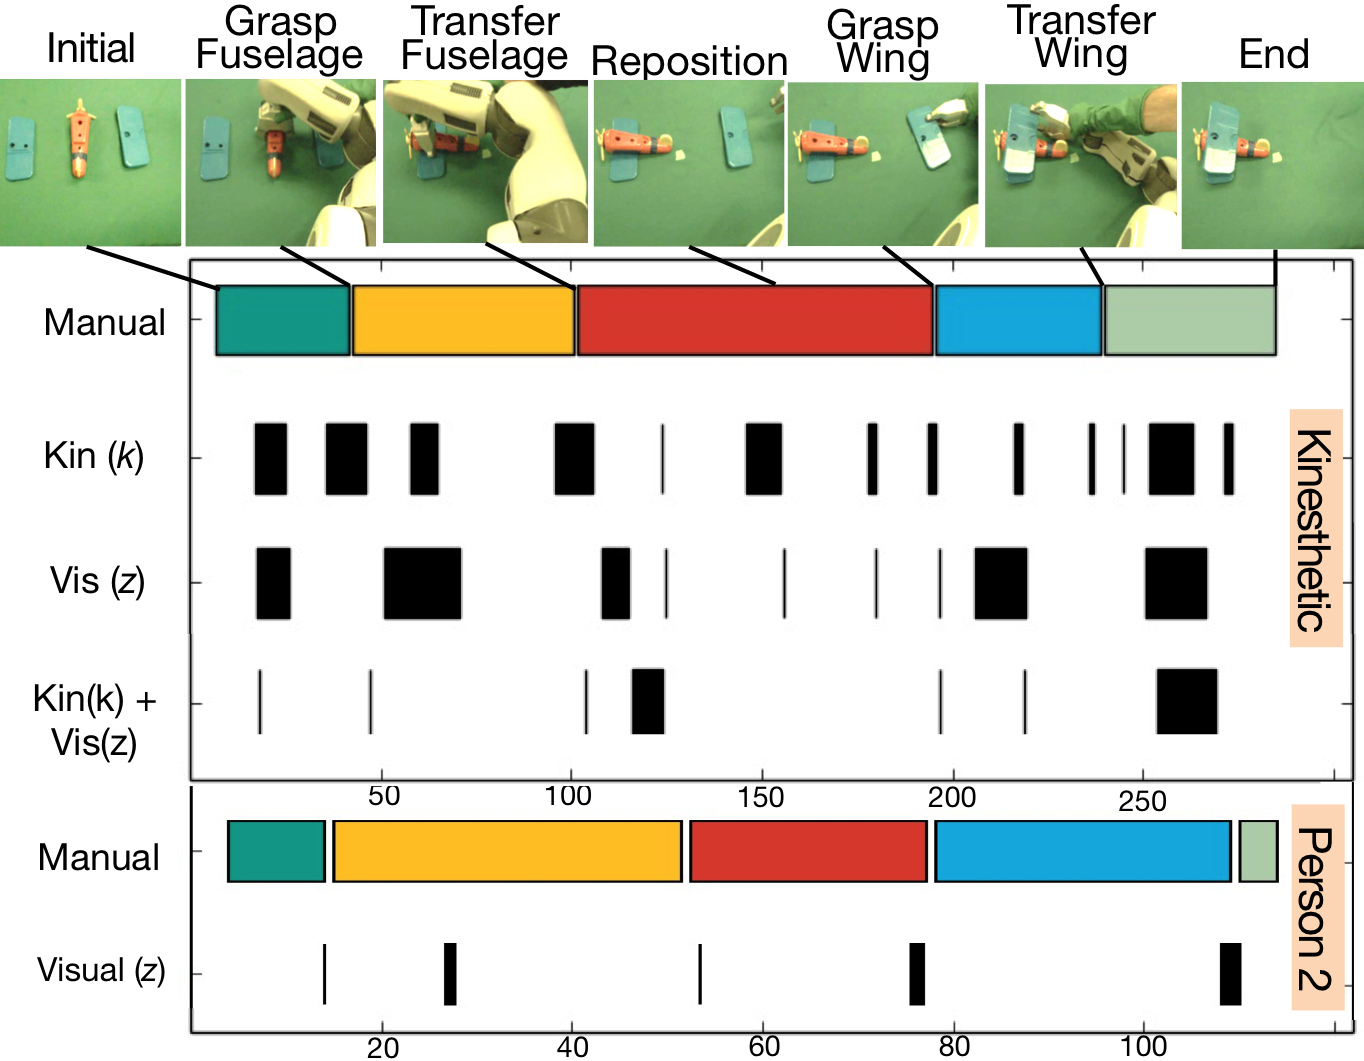
\includegraphics[width=\linewidth]{figures/pr2_plane_assembly.png}
\caption{The figure shows a sequence of images from the Toy Plane assembly (YCB Dataset). The first row shows a manual segmentation of the task in 4 semantic steps: Grasp Fuselage, Transfer Fuselage, Grasp Wing, Transfer Fuselage. Rows 2-4 show the sub-task level segmentation results from our completely unsupervised approach using 8 examples. Each row is a sequence of transitions represented by blocks. The width of every block represents the confidence interval conveying the length of transition, with some transitions being sharp while others are longer.}
 \label{fig:pr2_toyplane}
\vspace{-10pt} 
\end{figure}

While unsuperivsed segmentation has been widely studied in the context of kinematic data segmentation, increasingly, fixed camera video recordings accompany kinematic recordings of human teleoperation in a variety of datasets \cite{hodgins2009guide, gao2014jigsaws, ofli2013berkeley}.
The importance of visual sensing in segmentation has been suggested by experimental results in our prior work \cite{krishnan2015tsc} and by others \cite{Niekum2015learning}.
Visual features can provide crucial information in a number of scenarios: (1) a robot can only partially observe its state with kinematic data, (2) state-dependent sensor noise in a robots kinematic data, and (3) manipulations of objects in the environment.
However, existing unsupervised approaches rely on highly constrained visual sensing models: hand tuned features \cite{krishnan2015tsc}, poses for all objects in the workspace via AR markers \cite{Niekum2015learning}, or motion capture markers in human gesture extraction \cite{kulic2011incremental}.

In this work, we explore how we can relax these constraints by segmenting both kinematics and natural videos of demonstrations.
The key problem is leveraging raw visual data, i.e., pixels, due to the dimensionality and the featurization problem.
Fortunately, in computer vision, the growing maturity of \emph{deep} featurization e.g., Convolutional Neural Networks (CNNs), has led to a number of seminal results in visual feature extraction \cite{krizhevsky2012imagenet, lecun1995convolutional, jia2014caffe, long2014fully}.
Furthermore, frameworks like CAFFE \cite{jia2014caffe} allow for sharing pre-trained models (on terabyte-scale corpora of natural images), and this allows us to take advantage of these results even with relatively small datasets.

We explore an extension (\sys) to the Transition State Clustering algorithm \cite{krishnan2015tsc} with visual features.
At a high-level, this algorithm models demonstrations as switched linear dynamical systems.
It then identifies states at which regime transitions occur and clusters these states to identify regions of the state space associated with transitions.
The minimal covering set of transition clusters, i.e., clusters representing all demonstrations, gives a semantic segmentation for a task. 
We extend this framework by specifying the state space not only with kinematic states but also augmented with visual features.
Our experimental results surprisingly suggest that a time-series of frame-level visual features behave almost like smooth kinematic trajectories--satisfying the assumptions in our prior work.
Even with featurized videos, segmentation is not trivial, and there are a number of open questions including how to incorporate visual features into the model, how to navigate the number of hyperparameter and architecture choices, and the sufficiency of pre-trained networks.

We summarize the key experimental results.

\vspace{0.25em}

\textbf{Q0. Do generic visual features, deep or otherwise, improve segmentation accuracy? } While prior work in segmentation establishes that features from a constrained/hand-annotated visual sensing model can improve segmentation, an open question is whether there is enough information in natural videos with general-purpose features to improve segmentation accuracy. Our experimental results find that under partial kinematic observation and sensing noise, visual features dramatically improve segmentation accuracy by \textbf{x\%???}.

\vspace{0.25em}

\textbf{Q1. How do we transfer pre-trained neural network features to a very different domain? } Transfer learning of convolutional neural networks is an open problem in the computer vision community and a number of recent publications suggest caution or highly sensitive results \cite{oquab2014learning}.  These networks are trained on very different corpora of images than those seen in robotic demonstration videos. Even so, our results suggest that with the appropriate choice of convolutional layer to transfer, we can achieve accuracy improvements of \textbf{x\%???}.

\vspace{0.25em}

\textbf{Q2. How should visual features be incorporated into a kinematic segmentation model? } Even with automated featurization, the visual feature space is much higher dimensional than the kinematic state space. We explore dimensionality reduction techniques to mitigate some challenges due to the dimensionality. A natural approach would be to treat this problem as a multi-view manifold alignment problem e.g., finding a feature space maximally correlated with kinematics with Canonical Correlation Analysis. Surprisingly, our results suggest that this approach discards the novel information discovered by vision, and in fact random projections would do just as well (\textbf{x\%???}).

\vspace{0.25em}

\textbf{Q3. How do learned segmentations compare with human annotations? } We apply \sys to data from two datasets of surgical tasks \cite{gao2014jigsaws} where there were also human annotations of the same tasks.
While we find that \sys mostly agrees with the human annotations, there are a number of instances where \sys find crucial actions missed by the human annotators. (\textbf{List examples}) 

\iffalse
\begin{figure}[ht]
\centering
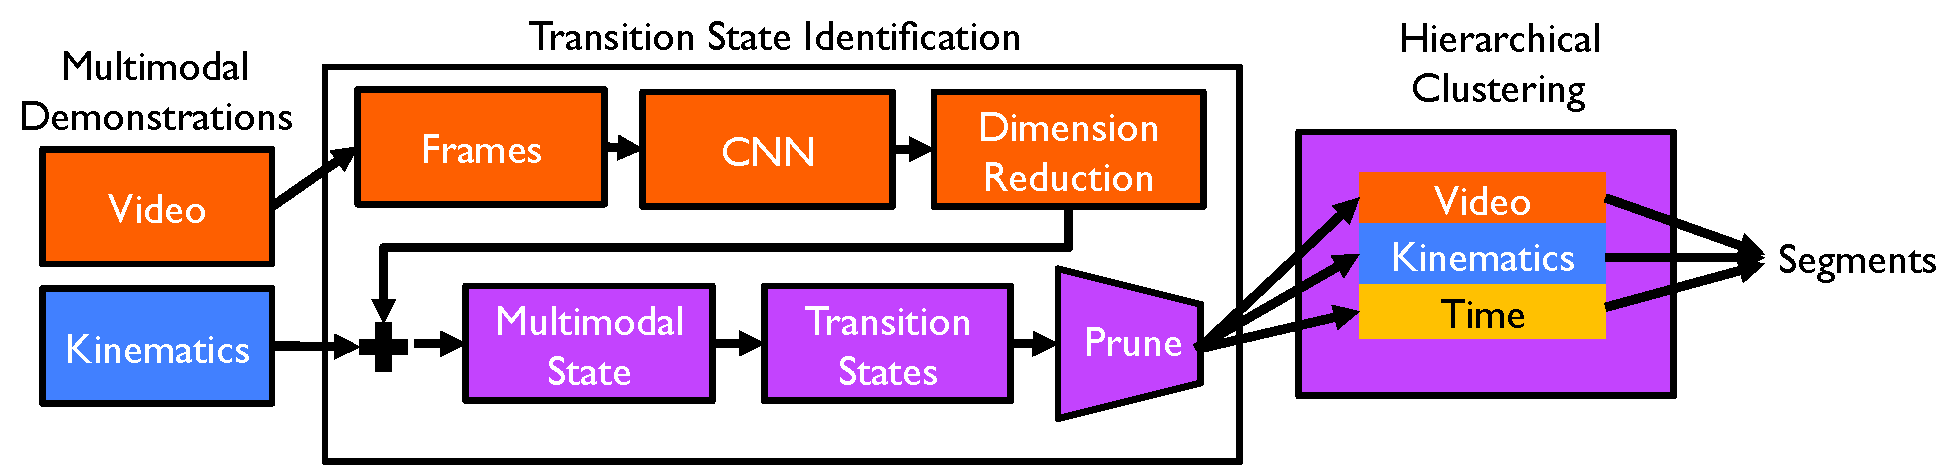
\includegraphics[width=\columnwidth]{figures/architecture.pdf}
\caption{\todo{name} architecture. We use a pre-trained CNN to featurize raw video data for use in segmentation. After featurization, we combine the data with kinematic data and apply a Transition State Clustering algorithm to identify segments. \label{fig:arch}}
\vspace{-1em}
\end{figure}
\fi

\section{Related Work}

\noindent\textbf{Surgical Segmentation: }

\begin{enumerate}
\item Describe ``surgeme" work
\end{enumerate}

\noindent\textbf{Segmentation in Other Robotics: }

\begin{enumerate}
\item Describe Neikum/others like DMP, GMM etc.
\end{enumerate}

\noindent\textbf{Related work in Computer Vision: }

\begin{enumerate}
\item Introduce Convolutional Network Research.
\end{enumerate}

\section{Problem Setup and Notation}
We first overview the Transition State Clustering algorithm.

\subsection{Transition State Clustering Model}
At a high-level, the Transition State Clustering algorithm (\sys), clusters states that mark dynamical regime transitions across all demonstrations.
This finds a discrete parametrization for transition events that can be used for segmentation.
In our prior work, we found that this model was more robust in comparison to alternatives.
We first outline the model, and then describe the algorithm to fit the parameters.

\subsubsection{Dynamical System Model}
Let $\mathcal{D}=\{d_i\}$ be the set of demonstrations where each $d_i$ is a trajectory $\mathbf{x}(t)=\binom{k(t)}{z(t)}$ of fully observed robot states and each state is a vector in $\mathbb{R}^d$.
$\mathbf{x}(t)$ encapsulates both the kinematic state $k(t)$ and a set of visual features $z(t)$.
We model each demonstration as a switched linear dynamical system.
There is a finite set of $d \times d$ matrices $\{A_1,...,A_k\}$, and an i.i.d zero-mean additive Gaussian Markovian noise process $W(t)$ which accounts for noise in the dynamical model:
\[
\mathbf{x}(t+1) = A_{i}\mathbf{x}(t) + W(t) \text{ : } A_i \in \{A_1,...,A_k\}
\]
In this model, transitions between regimes are instantaneous where each time $t$ is associated with exactly one dynamical system matrix $1,...,k$.

\subsubsection{Transition State Clusters}
Transition states are defined as the last states before a dynamical regime transition in \emph{each} demonstration.
Therefore, there will be times $t$ at which $A(t) \ne A(t+1)$.
A transition state is the state $x(t)$ at time $t$.
For a demonstration $i$, we denote the sequence of transitions states as $U_i=[u_i^1,...,u_i^J]$.
$J$ is the number of transition states where $J\ll T_i$ where $T_i$ is the time-length of $d_i$.

A \emph{transition state cluster} is
defined as a clustering of the set of transition states across all demonstrations; partitioning these transition states into $m$ non-overlapping similar groups:
\[
\mathcal{C} = \{C_1, C_2,...,C_m\}
\]
Every $U_i$ can be represented as a sequence of integers indicating that transition states assignment to one of the transition state clusters $U_i=[1,2,4,2]$.

We assume, demonstrations are \emph{consistent}, meaning there exists a non-empty sequence of transition states $\mathcal{U}^*$ such that the partial order defined by the elements in the sequence (i.e., $s_1$ happens before $s_2$ and $s_3$) is satisfied by every $U_i$. For example, 
\[U_1 = [1,3,4]\text{, }U_2 = [1,1,2,4]\text{, }\mathcal{U}^*=[1,4] \]
A counter example,
\[U_1 = [1,3,4]\text{, }U_2 = [2,5]\text{, }\mathcal{U}^*\text{  no solution} \]
Intuitively, this condition states that there have to be a consistent ordering of actions over all demonstrations up to some additional regimes (e.g., spurious actions). 
In case of multiple modes in an action sequence, we find the minimal consistent set.


\noindent \emph{Given a consistent set of demonstrations, the goal of the algorithm is to find a minimal solution, $\mathcal{U}^*$ that is loop free and respects the partial order of transitions in all demonstrations.}

\subsection{Transition State Clustering Algorithm}

\subsubsection{Transition State Identification}
The first step is to identify a set of transition states for each demonstration in $\mathcal{D}$.
Suppose there was only one regime, then this would be a linear regression problem:
\[
\arg\min_A \|A X_t - X_{t+1}\|
\]
where $X_t$ is a matrix where each column vector is $x(t)$, and $X_{t+1}$ is a matrix where each column vector is the corresponding $x(t+1)$.
Moldovan et al. \cite{moldovan2013dirichlet} proves that fitting a Jointly Gaussian model to $n(t) = \binom{\mathbf{x}(t+1)}{\mathbf{x}(t)}$ is equivalent to Bayesian Linear Regression.
We use Dirichlet Process Gaussian Mixture Models to learn the regimes without have to set the number of regimes in advance.
Each cluster learned signifies a different regime, and co-linear states are in the same cluster.
To find transition states, we move along a trajectory from $t=1,...,t_f$, and find states at which $n(t)$ is in a different cluster than $n(t+1)$.
These points mark a transition between clusters (i.e., transition regimes).

\subsubsection{Transition State Clustering}\label{prun}
Each of these regimes will have constituent vectors where each $n(t)$ belongs to a demonstration $d_i$. 
Transition states that mark transitions to or from regimes whose constituent vectors come from fewer than a fraction $\rho$ demonstrations are \emph{pruned}.
$\rho$ should be set based on the expected rarity of outliers.

After pruning, there are numerous transition states at different locations in the state-space.
If we model the states at transition states as drawn from a GMM model:
\[
{x}(t) \sim N(\mu_i, \Sigma_i)
\]
Then, we can apply the DP-GMM again to cluster the state vectors at the transition states.
Each cluster defines an ellipsoidal region of the state-space space.
The result of the pruning and clustering is a set of transition state clusters.

\subsection{Local Linearity of Visual Features}
We next describe why this model is still justified for the augmented state $\binom{k(t)}{z(t)}$.
In Figure \ref{fig:imgtraj}, for a single trajectory from one of our experimental datasets, we plot a 2D PCA visualization of the features from the first convolutional layer of a pre-trained AlexNet architecture. For each frame, we add a point to the visualization, illustrating the trajectory in feature space.
We see that the visual features follow a smooth trajectory even in the visual space. 

\begin{figure}[ht]
\centering
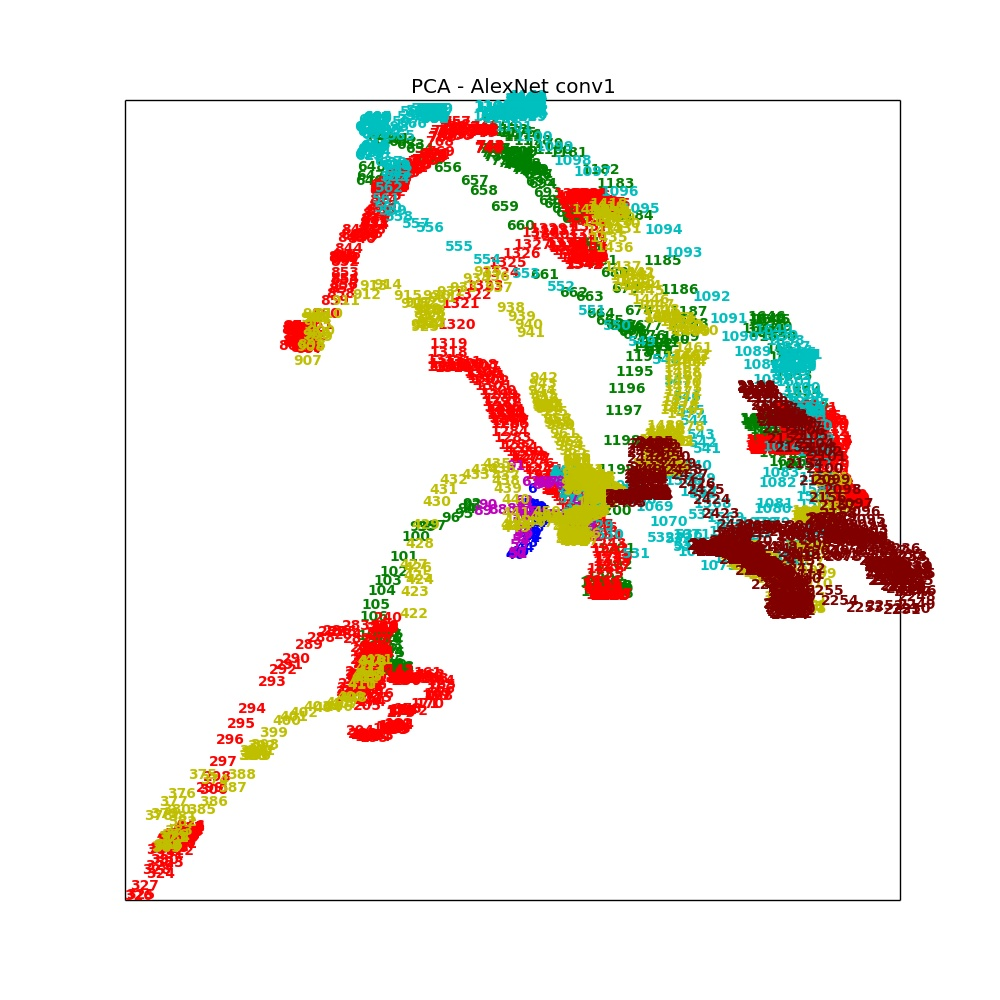
\includegraphics[width=\columnwidth]{figures/E5cap2_AlexNet_conv1_pca.jpg}
\caption{\todo{Fix image with more details, remove frame numbers and add points} \label{fig:imgtraj}}
\end{figure}

\begin{algorithm}[t!]
\small
\DontPrintSemicolon
\caption{\textbf{\TSC:} Visual-Transition State Clustering}
\KwData{Set of demonstrations:$\mathcal{D}$, $\rho$ pruning parameter}
\KwResult{Set of Predicted Transitions  $\mathcal{T}_i,\enspace \forall \, d_i \in \mathcal{D}$}
% \Begin{
    \ForEach{$d_i \in \mathcal{D}$}{
        $z_i \gets$ VisualFeatures $(d_i, params)$\;
        $k_i \gets$ KinematicFeatures $(d_i, params)$\;
        %  {\scriptsize  \tcp*[l]{concatenate kinematic and visual features}}
        $\mathbf{x}_i(t) \gets \binom{\mathbf{k_i}(t+1)}{\mathbf{z_i}(t)}\ \forall t \in \{1,\ldots, T_i\}$\;
        $\bar{x}_i(t) \gets \big[\, \mathbf{x}(t+1)^T, \ \mathbf{x}(t)^T, \ \mathbf{x}(t-1)^T \,\big]^T, \ \forall t$\;
        $N \gets \big[N^T, \bar{x}_i(1)^T,\ldots,\bar{x}_i(T_i)^T\big]^T$\;
    }
    {\scriptsize  \tcp*[l]{Cluster to get Change Points}}
    $\mathcal{C}^{CP} = \textnormal{DPGMM}(N, \alpha_0)$ {\scriptsize  \tcp*[r]{$\alpha_0$ is hyperparameter}}
    \ForEach{$N(n)\in\mathcal{C}^{CP}_{i},\ N(n+1)\in\mathcal{C}^{CP}_{j},i\neq j$ } {$CP \gets CP \cup \{N(n)\}$}
    {\scriptsize  \tcp*[l]{Cluster over Kinematic Feature Subspace}}
    $\mathcal{C}_{1} = \textnormal{DPGMM}(CP, \alpha_1)$ {\scriptsize  \tcp*[r]{$\mathcal{C}_{1}$: set of clusters}}
    %  \ForEach{$C^{1}_k \in \mathcal{C}^{1}$}{
    %     \uIf{$\sum_{d_i} \mathbbm{1}\Big( \sum_{n:N(n)\in d_i} \mathbbm{1}( CP(n) \in C^{1}_k) \geq 1 \Big) \geq \rho |\mathcal{D}|$}{
    %     $\mathcal{C}^{1}\gets \mathcal{C}^{1}\setminus \mathcal{C}^{1}_k$ {\scriptsize  \tcp*[r]{Cluster Pruning}}
    %     }
    %  }
    \ForEach{$C_{k} \in \mathcal{C}_{1}$}{
        $CP(C_{k}) \gets \{CP(n) \in C_{k}, \forall n \in \{1,\ldots,|CP|\}\}$\;
        {\scriptsize  \tcp*[l]{Cluster over Visual Feature Subspace}}
        $\mathcal{C}_{k2} \gets \textnormal{DPGMM}(CP(C_{k}), \alpha_2)$\;
        \ForEach{$C_{kk'} \in \mathcal{C}_{k2}$}{
            \If{$\sum_{d_i} \mathbbm{1}\Big( \sum_{n:N(n)\in d_i} \mathbbm{1}( CP(n) \in C_{kk'}) \geq 1 \Big) \leq \rho |\mathcal{D}|$}
            {$\mathcal{C}_{k2}\gets \mathcal{C}_{k2}\setminus \{C_{kk'}\}$ {\scriptsize \tcp*[r]{Cluster Pruning}}
            }
            {\scriptsize \tcp*[l]{collect intra-cluster transitions}}
            $T_i \gets T_i \cup \{CP(n) \in C^{kk'}, \forall n:N(n)\in d_i\}$\;
        }
    }
    {\scriptsize  \tcp*[l]{Cluster over time to predict Transition Windows}}
    \ForEach{$d_i \in \mathcal{D}$}{
        Repeat steps 1-17 for $\mathcal{D}' = \mathcal{D} \setminus d_i$\;
        $\mathtt{T}_j \gets \mathtt{T}_j \cup T_j^{(i)}, \ \{\forall\ j: d_j \in \mathcal{D}'\}${\scriptsize \tcp*[r]{$T_j^{(i)}$: \textit{i}th iteration}} 
        % $\mathcal{T}_i \gets DPGMM (\mathtt{T}, \alpha_4)${\scriptsize  \tcp*[r]{store cluster $\mu$ and $\Sigma$}}
    }
    \lForEach{$d_i \in \mathcal{D}$}{$\mathcal{T}_i \gets DPGMM (\mathtt{T}_i, \alpha_4)$}
    \nl\KwRet{$\mathcal{T}_i,\enspace \forall \, d_i \in \mathcal{D}$}
% }
\label{alg:vtsc}
\end{algorithm}

\section{Visual Transition State Clustering}
We present the \tsc algorithm in Algorithm~\ref{alg:vtrc}.
In this section, we overview the extensions to the previously proposed TSC algorithm~\cite{krishnan2015tsc}.

\subsection{Visual Features}
The first step in our extension is to define an augmented state space $\mathbf{x}(t) = \binom{k(t)}{z(t)}$, where $k(t)$ are the kinematic features and $z(t)$ are the visual features.
We use layers from a pre-trained Convolutional Neural Network (CNNs) to derive the features frame-by-frame.
CNNs are increasingly popular for image classification and as a result a number of image classification CNNs exist which are trained on terabytes of natural images.
Intuitively, CNNs are trained to classify based on aggregations (pools) of hierarchical convolutions of the pixels.
Removing the aggregations and the classifiers, results in convolutional filters which can be used to derive features.

However, we found that to use these features required a number of pre-processing and post-processing steps; in addition to a number of design choices within the CNN itself like what layer in the convolutional hierarchy to use.

\subsubsection{Pre-processing}
As the image classification CNNs are trained on static images, their features are optimized for identifying salient edges and colors.
Since these features are not temporal, they do not differentiate between robot and workspace features.
Furthermore, since we aggregate across demonstrations, we need to ensure that these features are largely consistent.
To avoid variance due to extraneous objects and small changes in lighting, we first pre-processed the videos.

We first cropped all videos by equal amounts to capture only the workspace where most of the robot manipulation happened. 
Then, they were rescaled to 640 x 480 dimensions with normalization to have a zero mean RGB value as standard \cite{krizhevsky2012imagenet,simonyan2014very}. 
Finally, for computational reasons, the videos were downsampled to \todo{x} frame per second.  
All of pre-processing happened with the open source program \texttt{ffmpeg}.

\subsubsection{Visual Featurization}
Once the images were pre-processed, we applied the convolutional filters from the pre-trained neural networks. In particular, we explore two architectures.

\vspace{0.25em}
\noindent\textbf{AlexNet: } Krizhevsky et al. proposed a convolutional neural network architecture for image classification \cite{krizhevsky2012imagenet}. This architecture was seminal as it proposed multiple stacked convolutional filters (5 in all).   

\vspace{0.25em}
\noindent\textbf{VGG: } Simoyan et al. proposed an alternative architecture termed VGG which increased the number of convolutional layers significantly (16 in all) \cite{simonyan2014very}.

\vspace{0.25em}

In this work, we explore selecting convolutional features from different layers in the hierarchy. 
This problem is called transfer learning and has been well studied \todo{cite}.
It is established that earlier layers in the hierarchy give more general features while later layers give more specific ones.
In our experiments, we explore the level of generality of features required for segmentation. 
We also compare these features to other visual featurization techniques such as SIFT and SURF.

\subsubsection{Post-Processing: Encoding}
After constructing these features, the next step is encoding the results of the convolutional filter into a vector $z(t)$.
We explore three encoding techniques: (1) raw values, (2) VLAD, and (3) LCD.

\vspace{0.25em}
\noindent\textbf{Raw Filter Values: } The first encoding technique that we explore is using the raw convolutional filter values. We stack these values into a vector which constructs $z(t)$.

\vspace{0.25em}
\noindent\textbf{Vector of Locally Aggregated Descriptors (VLAD)\cite{arandjelovic2013all}: }
Vector of Locally Aggregated Descriptors (VLAD) image encoding as proposed by is a feature encoding and pooling method. 
It transforms an incoming variable-size set of independent samples into a fixed size vector representation.
VLAD encodes a set of local feature descriptors $I=\{x_1,\ldots,x_n\}$ extracted from an image using a code book $\mathrm{C} = \{c_1, \ldots, c_K \}$ built using a clustering method. With K-coarse cluster centers, generated by K-means, we can obtain the difference vector for every center $c_j$ as:\vspace{-5pt}
\[ u_k = \sum_{i:\,1\text{-}nbd(x_i)=\{c_j\}} (x_i- c_j)
\]
where $k\text{-}nbd(x_i)$ indicates k(=1) nearest neighbors of $x_i$ among K coarse centers.
VLAD vector is obtained by concatenating $u_k$ over all the K centers, $V = [u_1^T, \ldots, u_K^T]$, with $V$ of size K$D$ where $D$ is the dimension of incoming points $x_i$. 

\vspace{0.25em}
\noindent\textbf{Latent Concept Descriptors (LCD) \cite{xu2014discriminative}: }
Convolutional layers contain important spatial information, however at the cost of high dimensional representation. For instance the feature dimension at a convolutional layer can be $c\times c \times M$, where $c$ is filter size and $M$ is number of filters. However using the latent concept descriptors, a layer of size $c\times c \times M$ can be converted into $c^2$ latent concept descriptors with M dimensions. Each latent concept descriptor represents the responses from the M filters for a specific pooling location. 

\subsubsection{Post-Processing: Dimensionality Reduction}
After encoding, we feed the features $z(t)$ through a dimensionality reduction process.
This is for computational reasons as the visual features are very high dimensional and the Transition State Clustering algorithm suffers from the curse of dimensionality.
Furthermore, almost all GMM-based clustering algorithms converge to a local minima and very high dimensional feature spaces can lead to numerical instability or inconsistent behavior.
Principal Component Analysis (PCA) is widely applied in computer vision. 
We explore alternative dimensionality reduction techniques to find desirable properties of the dimensionality reduction that result in improve segmentation performance.
In particular, we explore Gaussian Random Projections (GRP), and Canonical Correlation Analysis (CCA).

\subsection{Other Extensions}
\subsubsection{Sliding Window States}
In our prior work, we used the concatenation of kinematic and visual features at a given time $t$ as the state representation $\binom{k(t)}{z(t)}$. However, the use of rolling time window in both kinematics and visual space allows capturing dynamics. 
We empirically found that the use of $[k(t-1), k(t), k(t+1)]^T$ as the kinematic state representation led to improved segmentation accuracy. Other lengths of temporal history were experimented with as shown in Figure~\todo{add figure}.

\subsubsection{Skill-Weighted Pruning} 
Different demonstrators often have different skill levels, and we extend our prior work to prune transition states in a weighted way.
$w_i$ is weight for each demonstration $d_i \in \mathcal{D}$, such that $w_i \in [0,1]$ and $\hat{w}_i = \frac{w_i}{\sum w_i}$. Then a cluster $C_{kk'}$ is pruned if: 
\[\sum_{d_i} \hat{w}_i\mathbbm{1}\Big( \sum_{n:N(n)\in d_i} \mathbbm{1}( CP(n) \in C_{kk'}) \geq 1 \Big) \leq \rho 
\]

\subsubsection{Robust Temporal Clustering}
In our prior work, we used a hierarchical application of DP-GMM first clustering spatially and then temporally. 
In this work, we explore a more robust variant of this approach.
We iteratively hold out one out of the $N$ demonstrations and apply \tsc to the remaining demonstrations.
Then, over $N$ runs of $\tsc$, we temporally cluster the centroids of the transition state clusters.

% \vspace{0.5em}






% ==============================================

% \begin{algorithm}[t]
% \caption{The Transition State Clustering Algorithm \todo{Fix with changes} \label{algotext}}
% % \begin{algorithmic}[1]
% \scriptsize
% \State \textsf{Input: } $\mathcal{D}$, $\rho$ pruning parameter, and $\delta$ compaction parameter.

% \State $n(t) = \binom{\mathbf{x}(t+1)}{\mathbf{x}(t)}$. 

% \State Cluster the vectors $n(t)$ using DP-GMM assigning each state to its most likely cluster. 

% \State \emph{Transition states} are times when $n(t)$ is in a different cluster than $n(t+1)$. 

% \State Remove states that transition to and from clusters with less than a fraction of $p$ demonstrations. 

% \State Remove consecutive transition states when the L2 distance between these transitions is less than $\delta$. 

% \State Cluster the remaining transition states in the state space $\mathbf{x}(t+1)$ using DP-GMM.

% \State Within each state-space cluster, sub-cluster the transition states temporally. 

% \State \textsf{Output: } A set $\mathcal{M}$ of clusters of transition states and the associated with each cluster a time interval of transition times.
% % \end{algorithmic}
% \end{algorithm}


\documentclass[0-main.tex]{subfiles}
\begin{document}

\section{Experiments}
\label{sec:expt}

\begin{table}[t!]
\vspace{5pt}
\centering
\resizebox{\linewidth}{!}{% put in textwidth
\begin{tabular}{l|l|l|l}
\hline
\rowcolor[HTML]{CBCEFB} 
                 & \multicolumn{1}{c|}{GRP}          & \multicolumn{1}{c|}{PCA} &  \multicolumn{1}{c}{CCA}           \\ \hline \hline
SIFT             &          -     & 0.443$\pm$0.008 &        -     \\ %\hline
\rowcolor[HTML]{E0E0E0} 
AlexNet conv3     & 0.559$\pm$0.018  &  0.600$\pm$0.012  &  0.494$\pm$0.006  \\ %\hline 
AlexNet conv4     & 0.568$\pm$0.007  &  0.607$\pm$0.004  &  0.488$\pm$0.005  \\ %\hline
\rowcolor[HTML]{E0E0E0} 
AlexNet pool5     & 0.565$\pm$0.008  &  0.599$\pm$0.005  &  0.486$\pm$0.012  \\ %\hline
VGG conv5\_3      & 0.571$\pm$0.005  &  \textbf{0.637$\pm$0.009}  &  0.494$\pm$0.013  \\
\rowcolor[HTML]{E0E0E0} 
VGG LCD-VLAD       & 0.506$\pm$0.001  &  0.534$\pm$0.011  &  0.523$\pm$0.010  \\ %\hline
AlexNet LCD-VLAD   & 0.517$\pm$0.001  &  0.469$\pm$0.027  &  0.534$\pm$0.018  \\
\hline
\end{tabular}
}
\caption{The silhouette score for each of the techniques and dimensionality reduction schemes on a subset of suturing demonstrations (5 expert examples). We found that PCA (100 dims) applied to VGG conv5\_3 maximizes silhouette score  \label{tab:visual}}
\vspace{-10pt}
\end{table}


\subsection{Evaluation Metrics}\label{sec:metrics}
It is important to note that \tsc is an unsupervised algorithm that does not use labeling.
Therefore, we evaluate \tsc both intrinsically (without labels) and extrinsically (against human annotations).



\vspace{0.25em}
\noindent \textbf{Intrinsic metric:} The goal of the intrinsic metric is compare the performance of different featurization techniques, encodings, and dimensionality reduction within \tsc without reference to external labels.
This score is not meant to be an absolute metric of performance but rather a relative measure.
The intrinsic metric we use measures the ``tightness" of the transition state clusters. 
This metric is meaningful since we require that each transition state cluster contains transitions from a fraction of at least $\rho$ of the demonstrations, the tightness of the clusters measures how well \tsc discovers regions of the state space where transitions are grouped together.
This is measured with the mean \textit{Silhouette Score} (denoted by \textsf{ss}), which is defined as follows for each transition state $i$:  \vspace{-5pt}
\[ \textsf{ss}(i) = \frac{b(i) - a(i)}{max\{a(i), b(i)\}},\quad \textsf{ss}(i) \in [-1,1]
\]
if transition state $i$ is in cluster $C_j$, $a(i)$ is defined the average dissimilarity of point $i$ to all points in $C_j$, and $b(i)$ the dissimilarity with the closest cluster measured as the minimum mean dissimilarity of point $i$ to cluster $C_k,\ k\neq j$. We use $L_2$-norm as the dissimilarity metric and rescale \textsf{ss} $\in[0,1]$ for ease of comparison. 

\iffalse
\begin{figure}[!t]
\centering
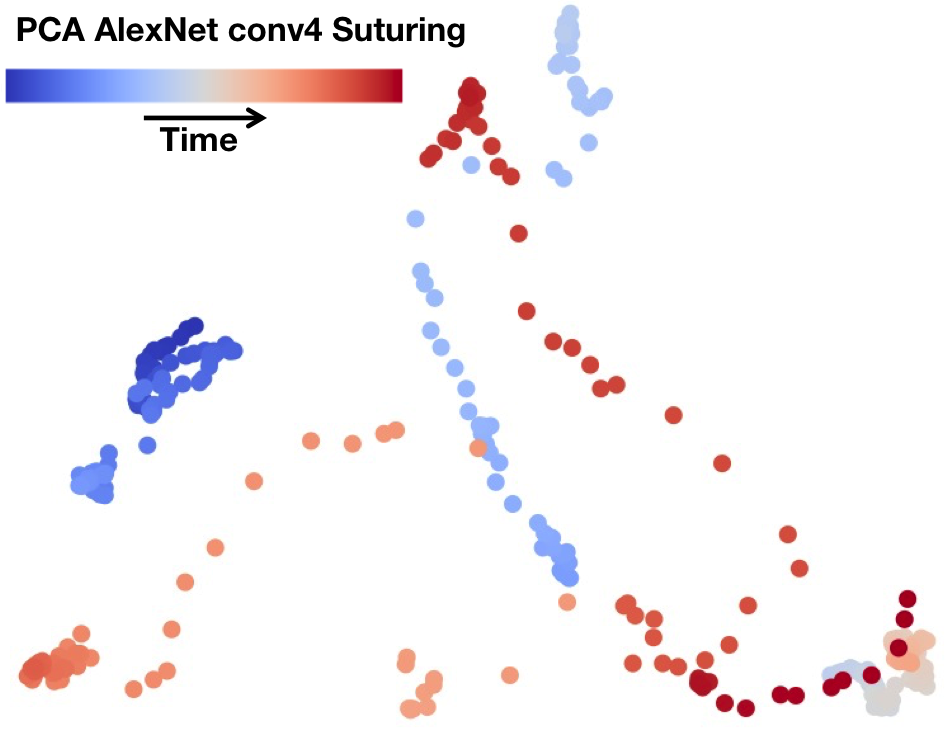
\includegraphics[width=0.5\linewidth]{figures/pca_conv4.png}
\caption{The figure visualizes the PCA projection of 64,896 dimensional output from \texttt{conv4} of the Alexnet for a sub-sequence of the suturing task video sub-sampled at 10 fps. The points are colored according to time from blue to red. We note that the visual features follow a smooth trajectory even in the high dimensional visual space. \todo{instead use a graph with knn for \% (y-axis) of time $X_{t-1}$\& $X_{t+1}$ for a given traj. at 10fps, are in k-nn with k$\in[2,30]$, rid of figure}  \label{fig:imgtraj}}
\vspace{-15pt}
\end{figure}
\fi

\begin{figure}[!b]
\vspace{-10pt}
\centering
    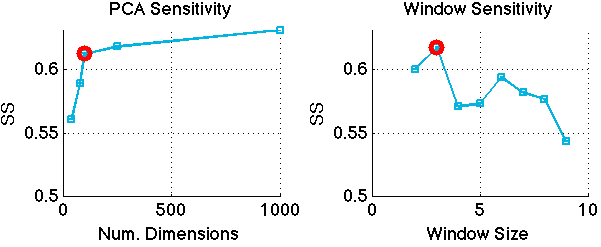
\includegraphics[width=0.95\linewidth]{figures/sensitivity}
    \caption{We evaluate the sensitivity of two hyperparameters set in advance: number of PCA dimensions and sliding window size. The selected value is shown in red double circles.\label{fig:sensitvity}}
\vspace{-10pt}
\end{figure}

\vspace{0.25em}
\noindent \textbf{Extrinsic metric:} To calculate an absolute measure of similarity of \tsc predictions $\mathcal{T}$ with respect to manual annotations $\mathcal{L}$, we use \textit{Normalized Mutual Information} (NMI) which measures the alignment between two label assignments. 
NMI is equal to the KL-divergence of the joint distribution with the product distribution of the marginals; intuitively, the distance from pairwise statistical independence.
% This metric captures the total error in alignment of predicted transitions to transitions in manual labels. 
NMI score lies in $[0,\ 1]$, where $0$ indicates independence while $1$  is perfect matching. It is defined as,
\[ NMI(\mathcal{T}, \mathcal{L}) = \frac{I(\mathcal{T}, \mathcal{L})}{\sqrt{H(\mathcal{T}) H(\mathcal{L})}}, \quad NMI(\mathcal{T}, \mathcal{L}) \in [0,1]
\]
% We compare similarity of predicted transitions to manual labels with the \textit{Dynamic Time Warping} distance between time-steps for transitions and manual labels. We normalize it by the temporal length of each example. This metric captures the total error in alignment of predicted transitions to transitions in manual labels. 

\subsection{Evaluation of Visual Featurization}
In our first experiment, we explore different visual featurization, encoding, and dimensionality reduction techniques.
We applied \tsc to our suturing experimental dataset, and measured the silhouette score of the resulting transition state clusters.
Table \ref{tab:visual} describes the featurization techniques on the vertical axis and dimensionality reduction techniques on the horizontal axis.
Our results suggest that on this dataset features extracted from the pre-trained CNNs resulted in tighter transition state clusters compared to SIFT features with a 3\% lower \textsf{ss} than the worst CNN result.
Next, we found that features extracted with the VGG architecture resulted in the highest \textsf{ss} with a 3\% higher \textsf{ss} than the best AlexNet result.
We also found that PCA for dimensionality reduction gave the best \textsf{ss} performance 7\% higher than the best GRP result and 10\% higher than best CCA result.
Because CCA finds projections of high correlation between the kinematics and video, we believe that CCA discard features informative features resulting in reduced clustering performance. 
We note that neither of the encoding schemes, VLAD or LCD\del{LCD$_{VLAD}$} significantly improve the \textsf{ss}.

\begin{figure}[!t]
\centering
%\begin{subfigure}[t]{4.4in}
    % \vspace{0pt}
    % \centering
    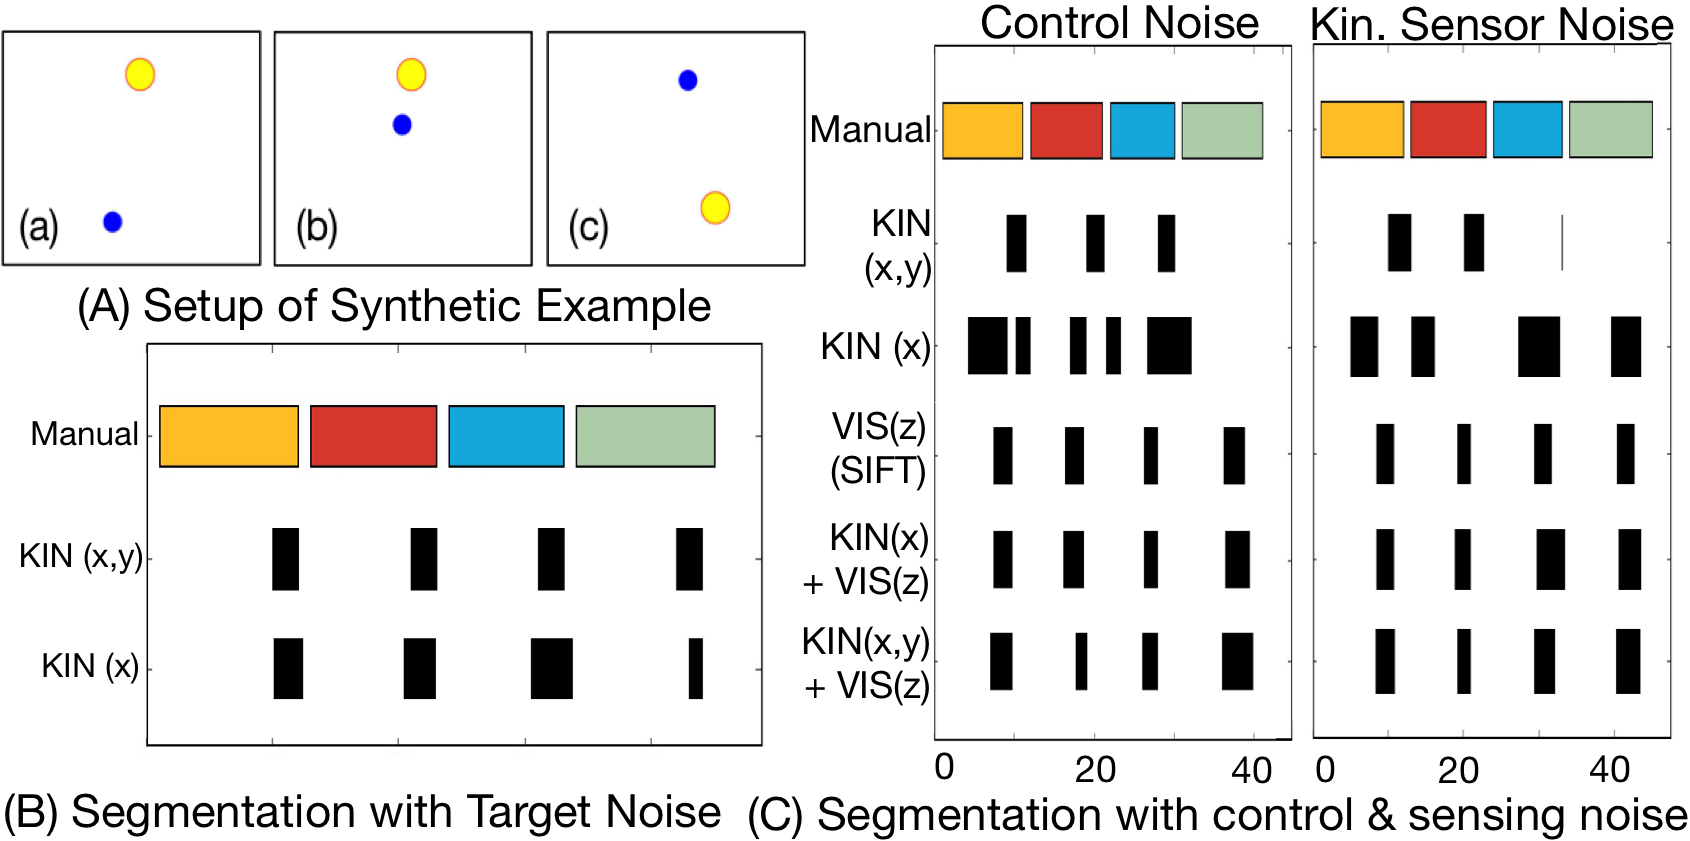
\includegraphics[width=\linewidth]{figures/toyEx-v3.png}
% 	\caption{Suturing}
% 	\par\vspace{0pt}
% 	\vspace{-15pt}
%\end{subfigure}
\caption{(A) The figure shows a 2D synthetic example with a moving point in blue and target in yellow. The robot moves to the target in a straight line in discrete steps, and a new target appears. 
(B) Segmentation results for repeated demonstrations with variance in target position.
(C) Segmentation under control noise, sensor noise, and partial observeration.}
\label{fig:toyEx}
\vspace{-10pt}
\end{figure}


There are two hyper-parameters for \tsc which we set empirically: sliding window size (T = 3), and the number of PCA dimensions (k = 100).
In Figure \ref{fig:sensitvity}, we show a sensitivity plot with the \textsf{ss} as a function of the parameter.
We calculated the \textsf{ss} using the same subset of the suturing dataset as above and with the VGG conv5\_3 CNN.
We found that T = 3 gave the best performance.
We also found that PCA with k = 1000 dimensions was only marginally better than k = 100 yet required $>$30 mins to run.
For computational reasons, we selected k = 100.




\iffalse
\subsubsection{Local Linearity of Visual Features}
In our first experiment, we explore whether the transitions state clustering model, originally derived for locally linear dynamical, is still justified for the augmented state $\mathbf{x}_(t) =\binom{k(t)}{z(t)}$.
In Figure \ref{fig:imgtraj}, for a single trajectory from one of our experimental datasets, we plot the percent if time, the points ($\mathbf{x}_(t-), \mathbf{x}_(t+1)$) lie within $k$-neighborhood of $\mathbf{x}_(t)$. We use the features from convolutional layer (\texttt{conv4}) of the pre-trained AlexNet. Higher values on y-axis for small $k$ represent that temporally consecutive points lie in vicinity in state space, even in the high dimensional visual space, supporting the assumptions of local linearity made by our model for identifying transitions.
\fi

% In Figure \ref{fig:imgtraj}, for a single trajectory from one of our experimental datasets, we plot a 2D PCA visualization of the features from convolutional layer (\texttt{conv4}) of the pre-trained AlexNet architecture. We use a sub-sequence of the full task and sub-sample the data at 10 fps and for each frame, we add a point to the visualization, illustrating the trajectory in feature space. It is worth noting that the visual features follow a smooth trajectory even in the high dimensional visual space, supporting the assumptions of local linearity made by our model for identifying transitions.

%\subsubsection{Encoding, Dimensionality Reduction, and Architecture}

\end{document}
\section{Latent State $H_t$}
Describe the process of linking kinematics and video (PCA, CCA, etc.).
If we apply any VLAD or encoding, or batching, describe it here:

\subsection{Temporal Batching}
We have so far used the concatenation of kinematic and visual features as the state representation $\binom{k(t)}{z(t)}$. However, the use of rolling time window in both kinematics and visual space allows capturing dynamics. Explicit use of first and second numerical derivatives in state representation for learning complex dynamics has been the state-of the art\tocite. 

We propose the use of a sequence raw states as the representation. Addition of every time step in the state implicitly corresponds to adding derivatives. However, the benefit of adding more time history saturates while the computational intensity requires scales quickly, especially with the use of high dimensional image features. 

We propose the use of $[k(t-1), k(t), k(t+1)]^T$ as the kinematic state representation. Other lengths of temporal history were experimented with as shown in Figure~\todo{add figure}. We note that while we use a 3 step temporal history, with data being captured at 30Hz, the amount of movement may be negligible between consecutive frames. We sub-sample the kinematic data to 10Hz to magnify kinematic changes. However, we keep the video data at 30Hz and use 9 consecutive frames for each $z(t)$. Using a CNN based featurization results in a very high dimensional feature vector, while use of SIFT like features results in a a feature vector of different lengths across different frames. Hence an encoding procedure as described following in employed to recover a concise and fixed dimensional representation for video subsequences. 

\todo{Current Status}: While batching is supposed to help in video analysis , I've seen good separation of clusters (PCA on conv features) with just individual frames without clustering... I think We need to look into this more and need to test it out with milestones clustering.


\subsection{Video Encoding}
Vector of Locally Aggregated Descriptors (VLAD) image encoding as proposed by \cite{arandjelovic2013all}\ignore{\cite{jegou2010aggregating}} is a feature encoding and pooling method, similar to Fisher vectors. 
It transforms an incoming variable-size set of independent samples into a fixed size vector representation.
VLAD was recently shown to perform better than Fisher vectors and average pooling for encoding multiple frames~\cite{xu2014discriminative}.

VLAD encodes a set of local feature descriptors $I=\{x_1,\ldots,x_n\}$ extracted from an image using a code book $\mathrm{C} = \{c_1, \ldots, c_K \}$ built using a clustering method such as Gaussian Mixture Models (GMM) or K-means clustering. With K-coarse cluster centers, generated by K-means, we can obtain the difference vector for every center $c_j$ as:
\[ u_k = \sum_{i:\,1\text{-}nbd(x_i)=\{c_j\}} (x_i- c_j)
\]
where $k\text{-}nbd(x_i)$ indicates k(=1) nearest neighbors of $x_i$ among K coarse centers.
VLAD vector is obtained by concatenating $u_k$ over all the K centers, $V = [u_1^T, \ldots, u_K^T]$, with $V$ of size K$D$ where $D$ is the dimension of incoming points $x_i$. 

Further, \cite{kantorov2014efficient} showed that VLAD-k, an extension to k-nearest neighbors outperforms vanilla VLAD (k=1). VLAD vectors are generally normalized using power normalization ($sign(u_k)\sqrt{\|u_k\|_2}$) followed by $L_2$ normalization of $V$. However an intra-normalization has been shown to perform better in balancing all the features~\cite{arandjelovic2013all}. This entails: $\hat{u}_k = u_k/\|u_k\|_2$ followed by $L_2$ normalization of $V$.
We use VLAD-k with k=5 followed by intra-normalization.

\subsection*{Latent Concept Descriptors}

It is worth noting that convolutional filters can be regarded as generalized linear classifiers on spatial patches, and each conv filter can be equated to a latent concept as proposed in~\cite{xu2014discriminative}. We represent the features from convolutional layers as vectors of latent concepts, with each entry representing a response to a latent concept. Since, conv filters at every layer are independent, each filter response can be understood as the prediction on linear classifier on respective latent concept.

Convolutional layers contain spatial information, however at the cost of high dimensional representation. For instance the feature dimension at a convolutional layer can be $c\times c \times M$, where $c$ is filter size and $M$ is number of conv filters. Simply flattening the layer would result in a high dimensional representation inducing computational instability. Since convolutional layers are higher dimensional than fully connected layers, they are often not used directly.

\todo{re-phrase}
However using the latent concept descriptors, a conv layer of size $c\times c \times M$ can be converted into $c^2$ latent concept descriptors with M dimensions. Each latent concept descriptor repre- sents the responses from the M filters for a specific pool- ing location. Once we obtain the latent concept descriptors for all the frames in a video, we then apply an encoding method to generate the video representation. In this case, each frame contains a2 descriptors instead of one descriptor for the frame.

\todo{Current Status}: We have also implemented the following encoding method- Latent Content Descriptors (LCD)+ VLAD \cite{xu2014discriminative}. However, initial results weren't super but we need to see how it performs on milestone clustering.

\subsection{Encoding Dimensionality}
The output of the encoding step is of the dimension $DK$, with D being the dimension of incoming points. Particularly in case of CNN features drawn from convolutional layers can run into tens of thousands leading to imbalance in the vectors after concatenation with kinematics. 

Hence 



\section{Results}
\subsection{Exp1. End-to-end result with some task}

\begin{enumerate}
\item Show that clusters are sensible and align with some intuitive criteria e.g., surgemes
\end{enumerate}

\subsection{Exp2. Does Vision Help}

\begin{enumerate}
\item Remove visual features and show that clusters degrade
\end{enumerate}

\subsection{Exp3. Parameter Search}

\begin{enumerate}
\item Describe our eval procedure and how we arrived at the architecture we did.
\end{enumerate}

\subsection{Exp4. Robustness}
\begin{enumerate}
\item Add noise or corrupt images and test to see how robust the segmentations we learn are.
\end{enumerate}


\subsection{Discussion}
\begin{enumerate}
\item How successful was our unsupervised approach in learning meaningful segmentations
\item RGB videos vs. RGB-D videos
\end{enumerate}


\section{Conclusion}
Summarize framework and results.


\subsubsection*{Acknowledgement}
This work is supported in part by a seed grant from the UC Berkeley CITRIS, and by the U.S.\ NSF Award IIS-1227536: Multilateral Manipulation by Human-Robot Collaborative Systems. We thank Intuitive Surgical, Simon DiMao, and the dVRK community for support; NVIDIA for computing equipment grants; Andy Chou and Susan Lim for developmental grants; and Sergey Levine and Katerina Fragkiadaki.


\bibliographystyle{IEEEtranS}
\bibliography{deepP2P}

\end{document}
